This subsection specifies the implementation details of the User Interface,
and should be considered together with figure \ref{fig:UI_views},
which illustrates the design proposed for the application.
The User Interface consists in a single page application,
divided into three main views: the \textit{Request}, \textit{Response} and \textit{Map view}.
Due to the implementation using React, every view is managed by a container,
which reads the state from the store, calls the rendering of presentational components,
and may dispatch actions on user input or other events. 

The User Interface is designed to be mobile friendly, by being responsive to the 
device size. This is achieved using the Bootstrap grid system, 
a website design paradigm in which the user screen is divided into 12 columns,
and each block of the user interface may specify a variable number of columns, depending on the screen size.
The results of this implementation is illustrated in figure \textbf{insert mobile vs desktop figure here}
%\ref{fig:desktop_vs_mobile_app},
where the mobile and desktop versions are put side a side for comparison.

Figure \ref{fig:user_interface_example} is a screenshot of the current version 
of developed application.


\begin{figure}[htpb]
  \centering
  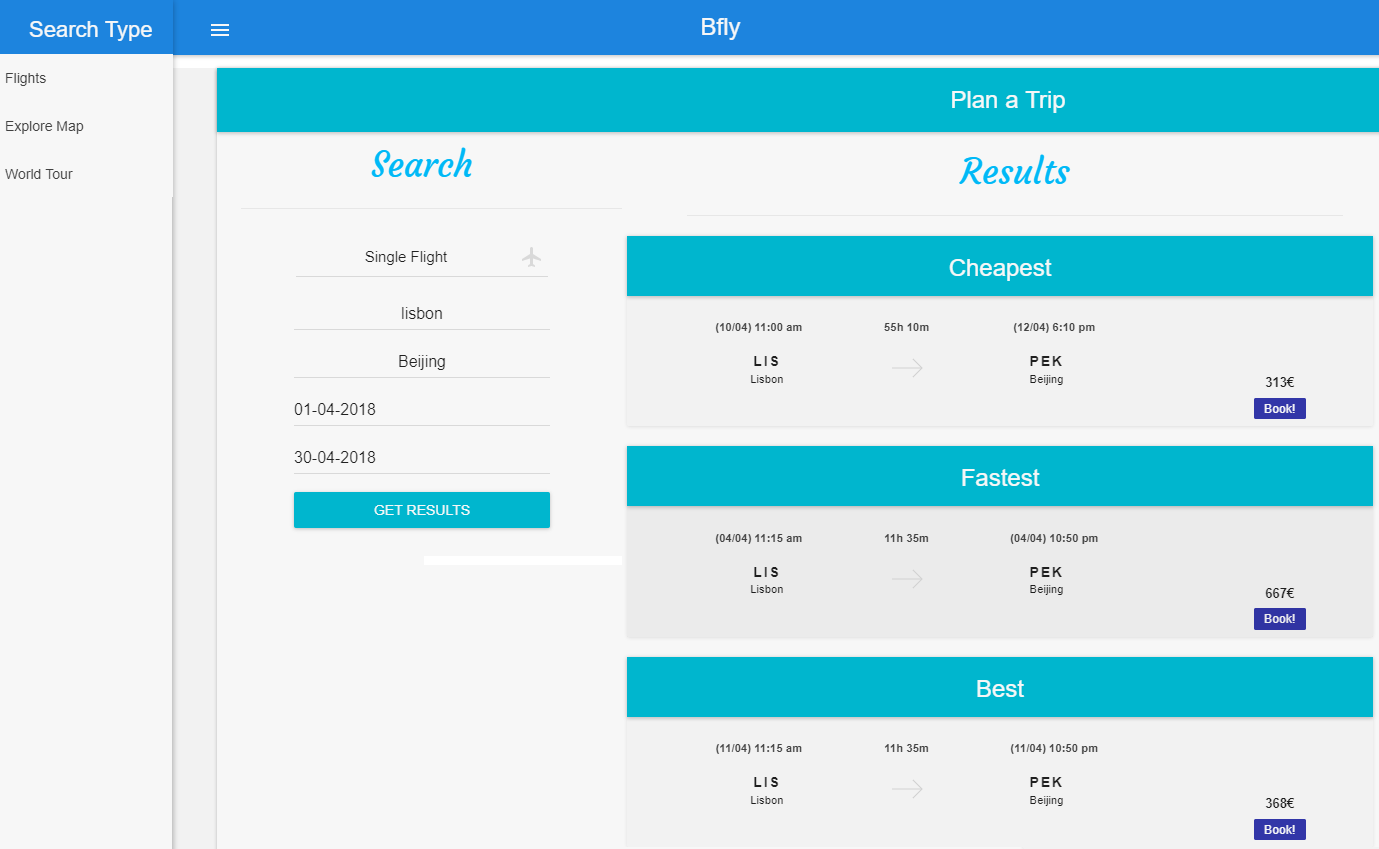
\includegraphics[width=\textwidth]{./Figures/system_implementation/user_interface_example.png}
  \caption{Print screen of the User Interface, as is, displaying the request 
  of a single flight between Lisbon and Beijing, over the span of a month. Three results 
  are presented, the cheapest (313€/55:10h), fastest (667€/11:35h), and most efficient (368€/11:35h) flight.}
  \label{fig:user_interface_example}  
\end{figure}